% Created by tikzDevice version 0.12.3.1 on 2022-09-02 10:49:52
% !TEX encoding = UTF-8 Unicode
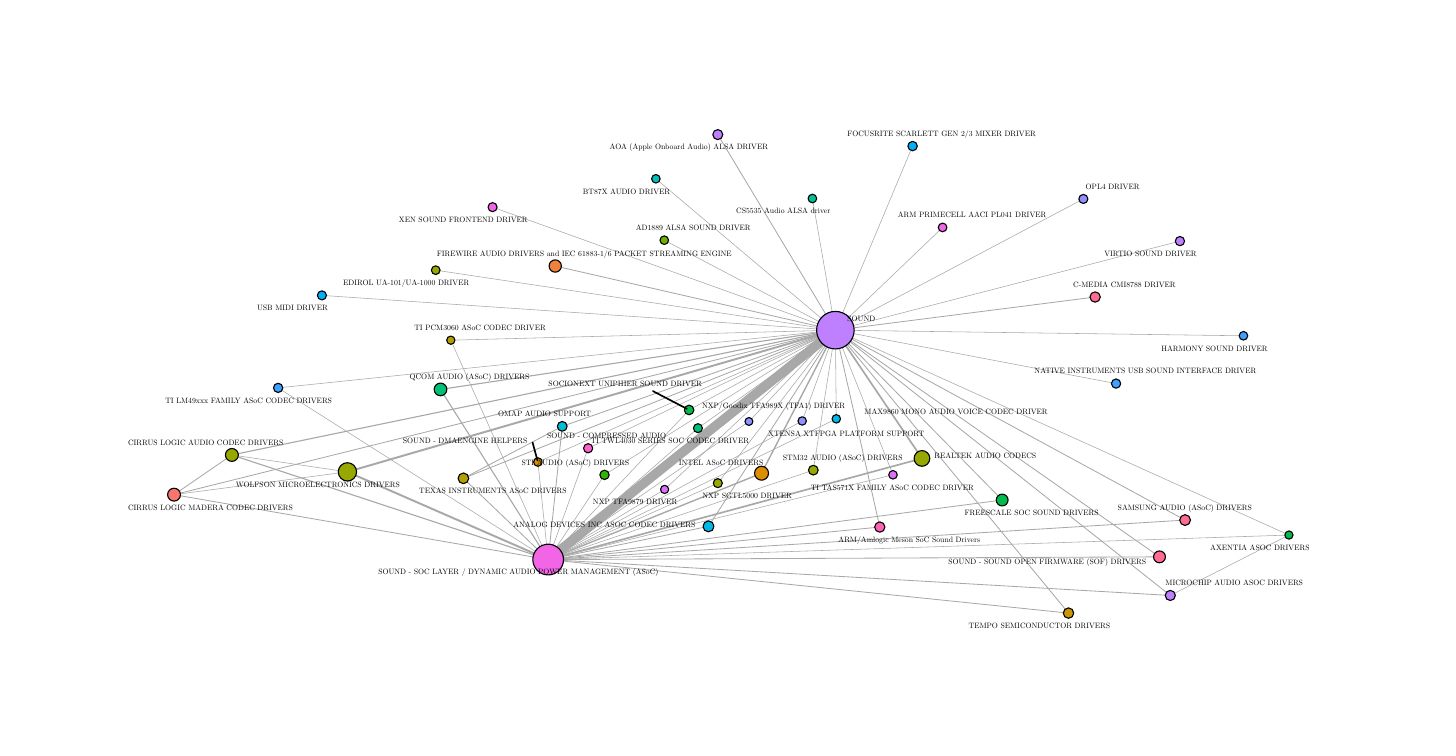
\begin{tikzpicture}[x=1pt,y=1pt]
\definecolor{fillColor}{RGB}{255,255,255}
\path[use as bounding box,fill=fillColor,fill opacity=0.00] (0,0) rectangle (505.89,252.94);
\begin{scope}
\path[clip] (  0.00,  0.00) rectangle (505.89,252.94);
\definecolor{fillColor}{RGB}{255,255,255}

\path[fill=fillColor] (  0.00,  0.00) rectangle (505.89,252.94);
\end{scope}
\begin{scope}
\path[clip] ( 32.75, 32.75) rectangle (475.89,222.94);
\definecolor{drawColor}{gray}{0.66}

\path[draw=drawColor,line width= 0.2pt,line join=round] (230.03,176.15) -- (291.86,143.63);

\path[draw=drawColor,line width= 0.3pt,line join=round] (246.01, 72.74) -- (291.86,143.63);

\path[draw=drawColor,line width= 0.3pt,line join=round] (246.01, 72.74) -- (188.08, 60.74);

\path[draw=drawColor,line width= 0.3pt,line join=round] (249.37,214.30) -- (291.86,143.63);

\path[draw=drawColor,line width= 0.2pt,line join=round] (330.60,180.75) -- (291.86,143.63);

\path[draw=drawColor,line width= 0.3pt,line join=round] (307.91, 72.49) -- (291.86,143.63);

\path[draw=drawColor,line width= 0.3pt,line join=round] (307.91, 72.49) -- (188.08, 60.74);

\path[draw=drawColor,line width= 0.2pt,line join=round] (455.75, 69.60) -- (412.88, 47.77);

\path[draw=drawColor,line width= 0.2pt,line join=round] (455.75, 69.60) -- (291.86,143.63);

\path[draw=drawColor,line width= 0.2pt,line join=round] (455.75, 69.60) -- (188.08, 60.74);

\path[draw=drawColor,line width= 0.2pt,line join=round] (227.00,198.34) -- (291.86,143.63);

\path[draw=drawColor,line width= 0.3pt,line join=round] (385.72,155.61) -- (291.86,143.63);

\path[draw=drawColor,line width= 0.3pt,line join=round] ( 73.79, 98.54) -- ( 52.89, 84.19);

\path[draw=drawColor,line width= 0.4pt,line join=round] ( 73.79, 98.54) -- (291.86,143.63);

\path[draw=drawColor,line width= 0.4pt,line join=round] ( 73.79, 98.54) -- (188.08, 60.74);

\path[draw=drawColor,line width= 0.2pt,line join=round] ( 73.79, 98.54) -- (115.54, 92.43);

\path[draw=drawColor,line width= 0.3pt,line join=round] ( 52.89, 84.19) -- (291.86,143.63);

\path[draw=drawColor,line width= 0.3pt,line join=round] ( 52.89, 84.19) -- (188.08, 60.74);

\path[draw=drawColor,line width= 0.2pt,line join=round] ( 52.89, 84.19) -- (115.54, 92.43);

\path[draw=drawColor,line width= 0.2pt,line join=round] (283.56,191.21) -- (291.86,143.63);

\path[draw=drawColor,line width= 0.2pt,line join=round] (147.45,165.31) -- (291.86,143.63);

\path[draw=drawColor,line width= 0.3pt,line join=round] (190.63,166.81) -- (291.86,143.63);

\path[draw=drawColor,line width= 0.2pt,line join=round] (319.76,210.16) -- (291.86,143.63);

\path[draw=drawColor,line width= 0.3pt,line join=round] (352.13, 82.25) -- (291.86,143.63);

\path[draw=drawColor,line width= 0.3pt,line join=round] (352.13, 82.25) -- (188.08, 60.74);

\path[draw=drawColor,line width= 0.2pt,line join=round] (439.32,141.60) -- (291.86,143.63);

\path[draw=drawColor,line width= 0.5pt,line join=round] (265.18, 91.94) -- (291.86,143.63);

\path[draw=drawColor,line width= 0.5pt,line join=round] (265.18, 91.94) -- (188.08, 60.74);

\path[draw=drawColor,line width= 0.2pt,line join=round] (292.19,111.59) -- (291.86,143.63);

\path[draw=drawColor,line width= 0.2pt,line join=round] (292.19,111.59) -- (188.08, 60.74);

\path[draw=drawColor,line width= 0.3pt,line join=round] (412.88, 47.77) -- (291.86,143.63);

\path[draw=drawColor,line width= 0.3pt,line join=round] (412.88, 47.77) -- (188.08, 60.74);

\path[draw=drawColor,line width= 0.2pt,line join=round] (393.29,124.33) -- (291.86,143.63);

\path[draw=drawColor,line width= 0.2pt,line join=round] (249.38, 88.35) -- (291.86,143.63);

\path[draw=drawColor,line width= 0.2pt,line join=round] (249.38, 88.35) -- (188.08, 60.74);

\path[draw=drawColor,line width= 0.2pt,line join=round] (230.16, 86.09) -- (291.86,143.63);

\path[draw=drawColor,line width= 0.2pt,line join=round] (230.16, 86.09) -- (188.08, 60.74);

\path[draw=drawColor,line width= 0.2pt,line join=round] (260.63,110.64) -- (291.86,143.63);

\path[draw=drawColor,line width= 0.2pt,line join=round] (260.63,110.64) -- (188.08, 60.74);

\path[draw=drawColor,line width= 0.3pt,line join=round] (193.16,108.88) -- (291.86,143.63);

\path[draw=drawColor,line width= 0.3pt,line join=round] (193.16,108.88) -- (188.08, 60.74);

\path[draw=drawColor,line width= 0.3pt,line join=round] (193.16,108.88) -- (157.45, 90.09);

\path[draw=drawColor,line width= 0.2pt,line join=round] (381.47,191.05) -- (291.86,143.63);

\path[draw=drawColor,line width= 0.4pt,line join=round] (149.17,122.22) -- (291.86,143.63);

\path[draw=drawColor,line width= 0.4pt,line join=round] (149.17,122.22) -- (188.08, 60.74);

\path[draw=drawColor,line width= 0.6pt,line join=round] (323.15, 97.29) -- (291.86,143.63);

\path[draw=drawColor,line width= 0.6pt,line join=round] (323.15, 97.29) -- (188.08, 60.74);

\path[draw=drawColor,line width= 0.3pt,line join=round] (418.23, 75.01) -- (291.86,143.63);

\path[draw=drawColor,line width= 0.3pt,line join=round] (418.23, 75.01) -- (188.08, 60.74);

\path[draw=drawColor,line width= 0.2pt,line join=round] (239.01,114.80) -- (291.86,143.63);

\path[draw=drawColor,line width= 0.2pt,line join=round] (239.01,114.80) -- (188.08, 60.74);

\path[draw=drawColor,line width= 0.2pt,line join=round] (291.86,143.63) -- (202.52,100.96);

\path[draw=drawColor,line width= 0.2pt,line join=round] (291.86,143.63) -- (184.37, 95.99);

\path[draw=drawColor,line width= 3.4pt,line join=round] (291.86,143.63) -- (188.08, 60.74);

\path[draw=drawColor,line width= 0.3pt,line join=round] (291.86,143.63) -- (408.98, 61.72);

\path[draw=drawColor,line width= 0.2pt,line join=round] (291.86,143.63) -- (208.44, 91.35);

\path[draw=drawColor,line width= 0.2pt,line join=round] (291.86,143.63) -- (283.89, 93.05);

\path[draw=drawColor,line width= 0.3pt,line join=round] (291.86,143.63) -- (376.10, 41.40);

\path[draw=drawColor,line width= 0.3pt,line join=round] (291.86,143.63) -- (157.45, 90.09);

\path[draw=drawColor,line width= 0.2pt,line join=round] (291.86,143.63) -- ( 90.50,122.78);

\path[draw=drawColor,line width= 0.2pt,line join=round] (291.86,143.63) -- (152.90,140.01);

\path[draw=drawColor,line width= 0.2pt,line join=round] (291.86,143.63) -- (312.68, 91.37);

\path[draw=drawColor,line width= 0.2pt,line join=round] (291.86,143.63) -- (242.19,108.22);

\path[draw=drawColor,line width= 0.2pt,line join=round] (291.86,143.63) -- (106.32,156.20);

\path[draw=drawColor,line width= 0.2pt,line join=round] (291.86,143.63) -- (416.36,175.81);

\path[draw=drawColor,line width= 0.7pt,line join=round] (291.86,143.63) -- (115.54, 92.43);

\path[draw=drawColor,line width= 0.2pt,line join=round] (291.86,143.63) -- (167.99,188.08);

\path[draw=drawColor,line width= 0.2pt,line join=round] (291.86,143.63) -- (279.87,110.82);

\path[draw=drawColor,line width= 0.2pt,line join=round] (202.52,100.96) -- (188.08, 60.74);

\path[draw=drawColor,line width= 0.2pt,line join=round] (184.37, 95.99) -- (188.08, 60.74);

\path[draw=drawColor,line width= 0.3pt,line join=round] (188.08, 60.74) -- (408.98, 61.72);

\path[draw=drawColor,line width= 0.2pt,line join=round] (188.08, 60.74) -- (208.44, 91.35);

\path[draw=drawColor,line width= 0.2pt,line join=round] (188.08, 60.74) -- (283.89, 93.05);

\path[draw=drawColor,line width= 0.3pt,line join=round] (188.08, 60.74) -- (376.10, 41.40);

\path[draw=drawColor,line width= 0.3pt,line join=round] (188.08, 60.74) -- (157.45, 90.09);

\path[draw=drawColor,line width= 0.2pt,line join=round] (188.08, 60.74) -- ( 90.50,122.78);

\path[draw=drawColor,line width= 0.2pt,line join=round] (188.08, 60.74) -- (152.90,140.01);

\path[draw=drawColor,line width= 0.2pt,line join=round] (188.08, 60.74) -- (312.68, 91.37);

\path[draw=drawColor,line width= 0.2pt,line join=round] (188.08, 60.74) -- (242.19,108.22);

\path[draw=drawColor,line width= 0.7pt,line join=round] (188.08, 60.74) -- (115.54, 92.43);

\path[draw=drawColor,line width= 0.2pt,line join=round] (188.08, 60.74) -- (279.87,110.82);
\definecolor{drawColor}{RGB}{0,0,0}
\definecolor{fillColor}{RGB}{113,176,0}

\path[draw=drawColor,line width= 0.4pt,line join=round,line cap=round,fill=fillColor] (230.03,176.15) circle (  1.55);
\definecolor{fillColor}{RGB}{0,183,232}

\path[draw=drawColor,line width= 0.4pt,line join=round,line cap=round,fill=fillColor] (246.01, 72.74) circle (  1.98);
\definecolor{fillColor}{RGB}{190,128,255}

\path[draw=drawColor,line width= 0.4pt,line join=round,line cap=round,fill=fillColor] (249.37,214.30) circle (  1.81);
\definecolor{fillColor}{RGB}{242,101,231}

\path[draw=drawColor,line width= 0.4pt,line join=round,line cap=round,fill=fillColor] (330.60,180.75) circle (  1.57);
\definecolor{fillColor}{RGB}{255,100,179}

\path[draw=drawColor,line width= 0.4pt,line join=round,line cap=round,fill=fillColor] (307.91, 72.49) circle (  1.86);
\definecolor{fillColor}{RGB}{0,187,75}

\path[draw=drawColor,line width= 0.4pt,line join=round,line cap=round,fill=fillColor] (455.75, 69.60) circle (  1.48);
\definecolor{fillColor}{RGB}{0,192,183}

\path[draw=drawColor,line width= 0.4pt,line join=round,line cap=round,fill=fillColor] (227.00,198.34) circle (  1.54);
\definecolor{fillColor}{RGB}{255,108,146}

\path[draw=drawColor,line width= 0.4pt,line join=round,line cap=round,fill=fillColor] (385.72,155.61) circle (  1.87);
\definecolor{fillColor}{RGB}{151,169,0}

\path[draw=drawColor,line width= 0.4pt,line join=round,line cap=round,fill=fillColor] ( 73.79, 98.54) circle (  2.33);
\definecolor{fillColor}{RGB}{248,118,109}

\path[draw=drawColor,line width= 0.4pt,line join=round,line cap=round,fill=fillColor] ( 52.89, 84.19) circle (  2.32);
\definecolor{fillColor}{RGB}{0,192,152}

\path[draw=drawColor,line width= 0.4pt,line join=round,line cap=round,fill=fillColor] (283.56,191.21) circle (  1.56);
\definecolor{fillColor}{RGB}{151,169,0}

\path[draw=drawColor,line width= 0.4pt,line join=round,line cap=round,fill=fillColor] (147.45,165.31) circle (  1.57);
\definecolor{fillColor}{RGB}{236,130,60}

\path[draw=drawColor,line width= 0.4pt,line join=round,line cap=round,fill=fillColor] (190.63,166.81) circle (  2.22);
\definecolor{fillColor}{RGB}{0,174,250}

\path[draw=drawColor,line width= 0.4pt,line join=round,line cap=round,fill=fillColor] (319.76,210.16) circle (  1.70);
\definecolor{fillColor}{RGB}{0,187,75}

\path[draw=drawColor,line width= 0.4pt,line join=round,line cap=round,fill=fillColor] (352.13, 82.25) circle (  2.13);
\definecolor{fillColor}{RGB}{61,161,255}

\path[draw=drawColor,line width= 0.4pt,line join=round,line cap=round,fill=fillColor] (439.32,141.60) circle (  1.55);
\definecolor{fillColor}{RGB}{221,141,0}

\path[draw=drawColor,line width= 0.4pt,line join=round,line cap=round,fill=fillColor] (265.18, 91.94) circle (  2.52);
\definecolor{fillColor}{RGB}{0,183,232}

\path[draw=drawColor,line width= 0.4pt,line join=round,line cap=round,fill=fillColor] (292.19,111.59) circle (  1.53);
\definecolor{fillColor}{RGB}{190,128,255}

\path[draw=drawColor,line width= 0.4pt,line join=round,line cap=round,fill=fillColor] (412.88, 47.77) circle (  1.83);
\definecolor{fillColor}{RGB}{61,161,255}

\path[draw=drawColor,line width= 0.4pt,line join=round,line cap=round,fill=fillColor] (393.29,124.33) circle (  1.67);
\definecolor{fillColor}{RGB}{151,169,0}

\path[draw=drawColor,line width= 0.4pt,line join=round,line cap=round,fill=fillColor] (249.38, 88.35) circle (  1.63);
\definecolor{fillColor}{RGB}{222,113,249}

\path[draw=drawColor,line width= 0.4pt,line join=round,line cap=round,fill=fillColor] (230.16, 86.09) circle (  1.48);
\definecolor{fillColor}{RGB}{143,145,255}

\path[draw=drawColor,line width= 0.4pt,line join=round,line cap=round,fill=fillColor] (260.63,110.64) circle (  1.43);
\definecolor{fillColor}{RGB}{0,189,209}

\path[draw=drawColor,line width= 0.4pt,line join=round,line cap=round,fill=fillColor] (193.16,108.88) circle (  1.77);
\definecolor{fillColor}{RGB}{143,145,255}

\path[draw=drawColor,line width= 0.4pt,line join=round,line cap=round,fill=fillColor] (381.47,191.05) circle (  1.64);
\definecolor{fillColor}{RGB}{0,191,118}

\path[draw=drawColor,line width= 0.4pt,line join=round,line cap=round,fill=fillColor] (149.17,122.22) circle (  2.29);
\definecolor{fillColor}{RGB}{151,169,0}

\path[draw=drawColor,line width= 0.4pt,line join=round,line cap=round,fill=fillColor] (323.15, 97.29) circle (  2.83);
\definecolor{fillColor}{RGB}{255,108,146}

\path[draw=drawColor,line width= 0.4pt,line join=round,line cap=round,fill=fillColor] (418.23, 75.01) circle (  1.95);
\definecolor{fillColor}{RGB}{0,187,75}

\path[draw=drawColor,line width= 0.4pt,line join=round,line cap=round,fill=fillColor] (239.01,114.80) circle (  1.73);
\definecolor{fillColor}{RGB}{190,128,255}

\path[draw=drawColor,line width= 0.4pt,line join=round,line cap=round,fill=fillColor] (291.86,143.63) circle (  6.78);
\definecolor{fillColor}{RGB}{254,97,207}

\path[draw=drawColor,line width= 0.4pt,line join=round,line cap=round,fill=fillColor] (202.52,100.96) circle (  1.66);
\definecolor{fillColor}{RGB}{221,141,0}

\path[draw=drawColor,line width= 0.4pt,line join=round,line cap=round,fill=fillColor] (184.37, 95.99) circle (  1.55);
\definecolor{fillColor}{RGB}{242,101,231}

\path[draw=drawColor,line width= 0.4pt,line join=round,line cap=round,fill=fillColor] (188.08, 60.74) circle (  5.55);
\definecolor{fillColor}{RGB}{255,108,146}

\path[draw=drawColor,line width= 0.4pt,line join=round,line cap=round,fill=fillColor] (408.98, 61.72) circle (  2.14);
\definecolor{fillColor}{RGB}{47,182,0}

\path[draw=drawColor,line width= 0.4pt,line join=round,line cap=round,fill=fillColor] (208.44, 91.35) circle (  1.69);
\definecolor{fillColor}{RGB}{151,169,0}

\path[draw=drawColor,line width= 0.4pt,line join=round,line cap=round,fill=fillColor] (283.89, 93.05) circle (  1.76);
\definecolor{fillColor}{RGB}{202,151,0}

\path[draw=drawColor,line width= 0.4pt,line join=round,line cap=round,fill=fillColor] (376.10, 41.40) circle (  1.88);
\definecolor{fillColor}{RGB}{179,160,0}

\path[draw=drawColor,line width= 0.4pt,line join=round,line cap=round,fill=fillColor] (157.45, 90.09) circle (  1.93);
\definecolor{fillColor}{RGB}{61,161,255}

\path[draw=drawColor,line width= 0.4pt,line join=round,line cap=round,fill=fillColor] ( 90.50,122.78) circle (  1.67);
\definecolor{fillColor}{RGB}{179,160,0}

\path[draw=drawColor,line width= 0.4pt,line join=round,line cap=round,fill=fillColor] (152.90,140.01) circle (  1.49);
\definecolor{fillColor}{RGB}{222,113,249}

\path[draw=drawColor,line width= 0.4pt,line join=round,line cap=round,fill=fillColor] (312.68, 91.37) circle (  1.54);
\definecolor{fillColor}{RGB}{0,191,118}

\path[draw=drawColor,line width= 0.4pt,line join=round,line cap=round,fill=fillColor] (242.19,108.22) circle (  1.62);
\definecolor{fillColor}{RGB}{0,174,250}

\path[draw=drawColor,line width= 0.4pt,line join=round,line cap=round,fill=fillColor] (106.32,156.20) circle (  1.64);
\definecolor{fillColor}{RGB}{190,128,255}

\path[draw=drawColor,line width= 0.4pt,line join=round,line cap=round,fill=fillColor] (416.36,175.81) circle (  1.67);
\definecolor{fillColor}{RGB}{151,169,0}

\path[draw=drawColor,line width= 0.4pt,line join=round,line cap=round,fill=fillColor] (115.54, 92.43) circle (  3.31);
\definecolor{fillColor}{RGB}{242,101,231}

\path[draw=drawColor,line width= 0.4pt,line join=round,line cap=round,fill=fillColor] (167.99,188.08) circle (  1.64);
\definecolor{fillColor}{RGB}{143,145,255}

\path[draw=drawColor,line width= 0.4pt,line join=round,line cap=round,fill=fillColor] (279.87,110.82) circle (  1.52);

\path[draw=drawColor,line width= 0.6pt,line join=round,line cap=round] (225.93,121.61) -- (238.20,115.22);

\path[draw=drawColor,line width= 0.6pt,line join=round,line cap=round] (182.44,103.05) -- (184.22, 96.54);

\node[text=drawColor,anchor=base,inner sep=0pt, outer sep=0pt, scale=  0.28] at (240.51,179.71) {AD1889 ALSA SOUND DRIVER};

\node[text=drawColor,anchor=base,inner sep=0pt, outer sep=0pt, scale=  0.28] at (208.40, 72.50) {ANALOG DEVICES INC ASOC CODEC DRIVERS};

\node[text=drawColor,anchor=base,inner sep=0pt, outer sep=0pt, scale=  0.28] at (238.92,208.81) {AOA (Apple Onboard Audio) ALSA DRIVER};

\node[text=drawColor,anchor=base,inner sep=0pt, outer sep=0pt, scale=  0.28] at (341.28,184.36) {ARM PRIMECELL AACI PL041 DRIVER};

\node[text=drawColor,anchor=base,inner sep=0pt, outer sep=0pt, scale=  0.28] at (318.59, 66.93) {ARM/Amlogic Meson SoC Sound Drivers};

\node[text=drawColor,anchor=base,inner sep=0pt, outer sep=0pt, scale=  0.28] at (445.26, 64.09) {AXENTIA ASOC DRIVERS};

\node[text=drawColor,anchor=base,inner sep=0pt, outer sep=0pt, scale=  0.28] at (216.39,192.82) {BT87X AUDIO DRIVER};

\node[text=drawColor,anchor=base,inner sep=0pt, outer sep=0pt, scale=  0.28] at (396.31,159.16) {C-MEDIA CMI8788 DRIVER};

\node[text=drawColor,anchor=base,inner sep=0pt, outer sep=0pt, scale=  0.28] at ( 64.34,102.07) {CIRRUS LOGIC AUDIO CODEC DRIVERS};

\node[text=drawColor,anchor=base,inner sep=0pt, outer sep=0pt, scale=  0.28] at ( 66.07, 78.65) {CIRRUS LOGIC MADERA CODEC DRIVERS};

\node[text=drawColor,anchor=base,inner sep=0pt, outer sep=0pt, scale=  0.28] at (273.05,185.70) {CS5535 Audio ALSA driver};

\node[text=drawColor,anchor=base,inner sep=0pt, outer sep=0pt, scale=  0.28] at (136.77,159.75) {EDIROL UA-101/UA-1000 DRIVER};

\node[text=drawColor,anchor=base,inner sep=0pt, outer sep=0pt, scale=  0.28] at (201.13,170.36) {FIREWIRE AUDIO DRIVERS and IEC 61883-1/6 PACKET STREAMING ENGINE};

\node[text=drawColor,anchor=base,inner sep=0pt, outer sep=0pt, scale=  0.28] at (330.26,213.72) {FOCUSRITE SCARLETT GEN 2/3 MIXER DRIVER};

\node[text=drawColor,anchor=base,inner sep=0pt, outer sep=0pt, scale=  0.28] at (362.78, 76.68) {FREESCALE SOC SOUND DRIVERS};

\node[text=drawColor,anchor=base,inner sep=0pt, outer sep=0pt, scale=  0.28] at (428.84,136.10) {HARMONY SOUND DRIVER};

\node[text=drawColor,anchor=base,inner sep=0pt, outer sep=0pt, scale=  0.28] at (250.59, 94.80) {INTEL ASoC DRIVERS};

\node[text=drawColor,anchor=base,inner sep=0pt, outer sep=0pt, scale=  0.28] at (335.46,113.29) {MAX9860 MONO AUDIO VOICE CODEC DRIVER};

\node[text=drawColor,anchor=base,inner sep=0pt, outer sep=0pt, scale=  0.28] at (435.99, 51.32) {MICROCHIP AUDIO ASOC DRIVERS};

\node[text=drawColor,anchor=base,inner sep=0pt, outer sep=0pt, scale=  0.28] at (403.88,127.91) {NATIVE INSTRUMENTS USB SOUND INTERFACE DRIVER};

\node[text=drawColor,anchor=base,inner sep=0pt, outer sep=0pt, scale=  0.28] at (259.97, 82.84) {NXP SGTL5000 DRIVER};

\node[text=drawColor,anchor=base,inner sep=0pt, outer sep=0pt, scale=  0.28] at (219.52, 80.55) {NXP TFA9879 DRIVER};

\node[text=drawColor,anchor=base,inner sep=0pt, outer sep=0pt, scale=  0.28] at (269.55,115.16) {NXP/Goodix TFA989X (TFA1) DRIVER};

\node[text=drawColor,anchor=base,inner sep=0pt, outer sep=0pt, scale=  0.28] at (186.76,112.50) {OMAP AUDIO SUPPORT};

\node[text=drawColor,anchor=base,inner sep=0pt, outer sep=0pt, scale=  0.28] at (392.04,194.59) {OPL4 DRIVER};

\node[text=drawColor,anchor=base,inner sep=0pt, outer sep=0pt, scale=  0.28] at (159.66,125.79) {QCOM AUDIO (ASoC) DRIVERS};

\node[text=drawColor,anchor=base,inner sep=0pt, outer sep=0pt, scale=  0.28] at (346.04, 97.29) {REALTEK AUDIO CODECS};

\node[text=drawColor,anchor=base,inner sep=0pt, outer sep=0pt, scale=  0.28] at (418.14, 78.62) {SAMSUNG AUDIO (ASoC) DRIVERS};

\node[text=drawColor,anchor=base,inner sep=0pt, outer sep=0pt, scale=  0.28] at (215.90,123.12) {SOCIONEXT UNIPHIER SOUND DRIVER};

\node[text=drawColor,anchor=base,inner sep=0pt, outer sep=0pt, scale=  0.28] at (301.24,146.68) {SOUND};

\node[text=drawColor,anchor=base,inner sep=0pt, outer sep=0pt, scale=  0.28] at (209.20,104.55) {SOUND - COMPRESSED AUDIO};

\node[text=drawColor,anchor=base,inner sep=0pt, outer sep=0pt, scale=  0.28] at (158.08,102.85) {SOUND - DMAENGINE HELPERS};

\node[text=drawColor,anchor=base,inner sep=0pt, outer sep=0pt, scale=  0.28] at (177.31, 55.21) {SOUND - SOC LAYER / DYNAMIC AUDIO POWER MANAGEMENT (ASoC)};

\node[text=drawColor,anchor=base,inner sep=0pt, outer sep=0pt, scale=  0.28] at (368.43, 58.95) {SOUND - SOUND OPEN FIRMWARE (SOF) DRIVERS};

\node[text=drawColor,anchor=base,inner sep=0pt, outer sep=0pt, scale=  0.28] at (197.91, 94.88) {STI AUDIO (ASoC) DRIVERS};

\node[text=drawColor,anchor=base,inner sep=0pt, outer sep=0pt, scale=  0.28] at (294.55, 96.61) {STM32 AUDIO (ASoC) DRIVERS};

\node[text=drawColor,anchor=base,inner sep=0pt, outer sep=0pt, scale=  0.28] at (365.60, 35.90) {TEMPO SEMICONDUCTOR DRIVERS};

\node[text=drawColor,anchor=base,inner sep=0pt, outer sep=0pt, scale=  0.28] at (168.13, 84.53) {TEXAS INSTRUMENTS ASoC DRIVERS};

\node[text=drawColor,anchor=base,inner sep=0pt, outer sep=0pt, scale=  0.28] at ( 79.86,117.26) {TI LM49xxx FAMILY ASoC CODEC DRIVERS};

\node[text=drawColor,anchor=base,inner sep=0pt, outer sep=0pt, scale=  0.28] at (163.47,143.57) {TI PCM3060 ASoC CODEC DRIVER};

\node[text=drawColor,anchor=base,inner sep=0pt, outer sep=0pt, scale=  0.28] at (312.42, 85.80) {TI TAS571X FAMILY ASoC CODEC DRIVER};

\node[text=drawColor,anchor=base,inner sep=0pt, outer sep=0pt, scale=  0.28] at (232.03,102.76) {TI TWL4030 SERIES SOC CODEC DRIVER};

\node[text=drawColor,anchor=base,inner sep=0pt, outer sep=0pt, scale=  0.28] at ( 95.67,150.62) {USB MIDI DRIVER};

\node[text=drawColor,anchor=base,inner sep=0pt, outer sep=0pt, scale=  0.28] at (405.74,170.31) {VIRTIO SOUND DRIVER};

\node[text=drawColor,anchor=base,inner sep=0pt, outer sep=0pt, scale=  0.28] at (104.85, 86.87) {WOLFSON MICROELECTRONICS DRIVERS};

\node[text=drawColor,anchor=base,inner sep=0pt, outer sep=0pt, scale=  0.28] at (157.43,182.56) {XEN SOUND FRONTEND DRIVER};

\node[text=drawColor,anchor=base,inner sep=0pt, outer sep=0pt, scale=  0.28] at (295.76,105.27) {XTENSA XTFPGA PLATFORM SUPPORT};
\end{scope}
\end{tikzpicture}
